\usepackage{amsmath}
\usepackage{amsfonts,amssymb,amsthm,color,dsfont,amsbsy}
\usepackage{mathrsfs}

\usepackage[T1]{fontenc}
\usepackage{mlmodern} 

\usepackage{caption}
\captionsetup{labelsep=period}

%========================================
% Add dot to section number (for article class)
%========================================
\renewcommand{\thesection}{\arabic{section}}
\makeatletter
\renewcommand{\@seccntformat}[1]{\csname the#1\endcsname.\ }  % add dot visually
\makeatother

\makeatletter
\def\numberline#1{\hb@xt@\@tempdima{#1.\hfil}}
\makeatother
%========================================
\usepackage[dvipsnames]{xcolor} 
\definecolor{bleudefrance}{rgb}{0.19, 0.35, 0.9}
\newcommand\blue[1]{{\color{bleudefrance}{#1}}}

\usepackage{geometry}
\geometry{  a4paper,
  hcentering,
  textwidth=0.68\paperwidth,
  top=0.16\paperheight,
  bottom=30mm}

\usepackage{hyperref}
\hypersetup{
  colorlinks = true,
  allcolors = blue,
}

%\renewcommand{\baselinestretch}{1.05}
\usepackage[all, knot, color]{xy}

% \usepackage{marginnote}
% \usepackage{bbold}
% \usepackage{changepage}
\usepackage{amscd}
% \usepackage{showframe}
% \usepackage[inner]{showlabels}
\usepackage{mathtools}
\usepackage{bm}
\usepackage{eucal}
\usepackage{extpfeil}
\usepackage{float}


\usepackage{tikz}
\usetikzlibrary{cd, calc, knots}
\usetikzlibrary{shapes.geometric}
\usetikzlibrary{decorations, decorations.markings} 
\usetikzlibrary{arrows, arrows.meta}
\tikzset{
    partial ellipse/.style args={#1:#2:#3}{
        insert path={+ (#1:#3) arc (#1:#2:#3)}
    }
}

\tikzset{->-/.style={decoration={
markings,
mark=at position #1 with {\arrow{>}}},postaction={decorate}}}
\tikzset{-<-/.style={decoration={
markings,
mark=at position #1 with {\arrow{<}}},postaction={decorate}}}
\tikzset{-<<-/.style={decoration={
markings,
mark=at position #1 with {\arrow{-latex}}},postaction={decorate}}}

\usepackage{graphicx}

\usepackage{enumitem}
\setlist[enumerate,1]{label={\rm (\alph*)}, topsep=.2em, noitemsep=1em, leftmargin=35pt, labelsep=7pt}
% \usepackage{quiver}
%%%%%%%%%%%%%%%%%%%%%%%%%%%%%%%%%%%%%%%%%%%%%%%%%%%%%%%%%%%%
% Environments (for amsbook)
%%%%%%%%%%%%%%%%%%%%%%%%%%%%%%%%%%%%%%%%%%%%%%%%%%%%%%%%%%%% 
% \usepackage{chngcntr}
% % Continuous section numbering
% \counterwithout{section}{chapter}

% \makeatletter
% \newtheoremstyle{amsart-like}
%   {3pt}                 % Space above
%   {3pt}                 % Space below
%   {\itshape}            % Body font
%   {}                    % Indent
%   {\bfseries}           % Head font
%   {.}                   % Punctuation
%   {5pt plus 1pt minus 1pt} % Space after head
%   {\thmname{#1}\thmnumber{ #2}\thmnote{ (#3)}} % Head spec
% \makeatother

% % Apply the style
% \theoremstyle{amsart-like}
% \newtheorem{theorem}{Theorem}[section] % Number by section
% \newtheorem{thm}[theorem]{Theorem}
% \newtheorem{lemma}[theorem]{Lemma}     % Share numbering
% \newtheorem{cor}[theorem]{Corollary}
% \newtheorem{corollary}[theorem]{Corollary}
% \newtheorem{prop}[theorem]{Proposition}
% \newtheorem{proposition}[theorem]{Proposition}
% \newtheorem{sublemma}[theorem]{Sublemma}
% \newtheorem{remarks}[theorem]{Remarks}
% \newtheorem{question}[theorem]{Question}
% \newtheorem*{basic}{Basic Question}

% \makeatletter
% \newtheoremstyle{amsart-definition}
%   {3pt}                 % Space above
%   {3pt}                 % Space below
%   {}            % Body font (italic)
%   {}                    % Indent
%   {\bfseries}           % Head font (bold)
%   {.}                   % Punctuation after head
%   {5pt plus 1pt minus 1pt} % Space after head
%   {\thmname{#1}\thmnumber{ #2}\thmnote{ (#3)}} % Note formatting
% \makeatother

% \theoremstyle{amsart-definition}
% \newtheorem{exmp}[theorem]{Example}
% \newenvironment{example}{\renewcommand{\qedsymbol}{\Large $\blacksquare$}\pushQED{\qed}\exmp}{\popQED\endexmp}
% \newtheorem{excs}[theorem]{Exercise}
% \newtheorem{defn}[theorem]{Definition}
% \newenvironment{definition}{\renewcommand{\qedsymbol}{\Large $\blacksquare$}\pushQED{\qed}\defn}{\popQED\enddefn}
% \newtheorem{rmk}[theorem]{Remark}
% \newenvironment{remark}{\renewcommand{\qedsymbol}{\Large $\blacksquare$}\pushQED{\qed}\rmk}{\popQED\endrmk}
% \newtheorem{fact}[theorem]{Fact}
% \newtheorem{obs}[theorem]{Observation}
% \newenvironment{observation}{\renewcommand{\qedsymbol}{\Large $\blacksquare$}\pushQED{\qed}\obs}{\popQED\endobs}
% \newtheorem{conv}[theorem]{Convention}

% % --- Force parentheses around optional notes ---
% \usepackage{etoolbox}
% \makeatletter
% \patchcmd{\@thm}{\thm@head@punct}{\thm@head@punct\ (}{}{} % Add '(' before note
% \patchcmd{\@endtheorem}{\@endparenv}{\ignorespacesafterend\ )\@endparenv}{}{} % Add ')' after note
% \makeatother

%%%%%%%%%%%%%%%%%%%%%%%%%%%%%%%%%%%%%%%%%%%%%%%%%%%%%%%%%%%%
% Environments (for amsart)
%%%%%%%%%%%%%%%%%%%%%%%%%%%%%%%%%%%%%%%%%%%%%%%%%%%%%%%%%%%% 
\newtheorem{thm}{Theorem}[section]
\newtheorem{theorem}{thm}[section]
\newtheorem{cor}[thm]{Corollary}
\newtheorem{corollary}[thm]{Corollary}
\newtheorem{prop}[thm]{Proposition}
\newtheorem{proposition}[thm]{Proposition}
\newtheorem{lemma}[thm]{Lemma}
\newtheorem{sublemma}[thm]{Sublemma}
\newtheorem{remarks}[thm]{Remarks}
\newtheorem{question}[thm]{Question}
\newtheorem*{basic}{Basic Question}

\theoremstyle{definition}
\newtheorem{exmp}[thm]{Example}
\newenvironment{example}{\renewcommand{\qedsymbol}{$\blacksquare$}\pushQED{\qed}\exmp}{\popQED\endexmp}
\newtheorem{excs}[thm]{Exercise}
\newtheorem{defn}[thm]{Definition}
\newenvironment{definition}{\renewcommand{\qedsymbol}{$\blacksquare$}\pushQED{\qed}\defn}{\popQED\enddefn}
\newtheorem{rmk}[thm]{Remark}
\newenvironment{remark}{\renewcommand{\qedsymbol}
{$\blacksquare$}\pushQED{\qed}\rmk}{\popQED\endrmk}
\newtheorem{fact}[thm]{Fact}
\newtheorem{obs}[thm]{Observation}
\newenvironment{observation}{\renewcommand{\qedsymbol}{$\blacksquare$}\pushQED{\qed}\obs}{\popQED\endobs}
\newtheorem{conv}[thm]{Convention}
\renewcommand{\theequation}{\thesection.\arabic{equation}}
\renewcommand{\theequation}{\thechapter.\arabic{equation}}
\numberwithin{equation}{section}

\def\proj{\operatorname{Proj}}
\def\mtr{\mathbf{t}}
%%%%%%%%%%%%%%%%%%%%%%%%%%%%%%%%%%%%%%%%%%%%%%%%%%%%%%%%%%%%
% Cal
%%%%%%%%%%%%%%%%%%%%%%%%%%%%%%%%%%%%%%%%%%%%%%%%%%%%%%%%%%%% 
\def\cA{\mathcal{A}}
\def\cB{\mathcal{B}}
\def\cC{\mathcal{C}}
\def\cD{\mathcal{D}}
\def\cE{\mathcal{E}}
\def\cF{{\mathcal{F}}}
\def\cG{{\mathcal{G}}}
\def\cH{\mathcal{H}}
\def\cI{\mathcal{I}}
\def\cJ{\mathcal{J}}
\def\cK{\mathcal{K}}
\def\cL{\mathcal{L}}
\def\cM{\mathcal{M}}
\def\cN{\mathcal{N}}
\def\cO{\mathcal{O}}
\def\cP{\mathcal{P}}
\def\cQ{\mathcal{Q}}
\def\cR{\mathcal{R}}
\def\cS{\mathcal{S}}
\def\cT{\mathcal{T}}
\def\cU{\mathcal{U}}
\def\cV{\mathcal{V}}
\def\cW{\mathcal{W}}
\def\cX{\mathcal{X}}
\def\cY{\mathcal{Y}}
\def\cZ{\mathcal{Z}}
%%%%%%%%%%%%%%%%%%%%%%%%%%%%%%%%%%%%%%%%%%%%%%%%%%%%%%%%%%%%
% BB
%%%%%%%%%%%%%%%%%%%%%%%%%%%%%%%%%%%%%%%%%%%%%%%%%%%%%%%%%%%% 
\def\bA{{\mathbb{A}}}
\def\bB{{\mathbb{B}}}
\def\bC{{\mathbb{C}}}
\def\bD{{\mathbb{D}}}
\def\bE{{\mathbb{E}}}
\def\bF{{\mathbb{F}}}
\def\bG{{\mathbb{G}}}
\def\bH{{\mathbb{H}}}
\def\bI{{\mathbb{I}}}
\def\bJ{{\mathbb{J}}}
\def\bK{{\mathbb{K}}}
\def\bL{{\mathbb{L}}}
\def\bM{{\mathbb{M}}}
\def\bN{{\mathbb{N}}}
\def\bO{{\mathbb{O}}}
\def\bP{{\mathbb{P}}}
\def\bQ{{\mathbb{Q}}}
\def\bR{{\mathbb{R}}}
\def\bS{{\mathbb{S}}}
\def\bT{{\mathbb{T}}}
\def\bU{{\mathbb{U}}}
\def\bV{{\mathbb{V}}}
\def\bW{{\mathbb{W}}}
\def\bX{{\mathbb{X}}}
\def\bY{{\mathbb{Y}}}
\def\bZ{{\mathbb{Z}}}
%%%%%%%%%%%%%%%%%%%%%%%%%%%%%%%%%%%%%%%%%%%%%%%%%%%%%%%%%%%%
% Bold math
%%%%%%%%%%%%%%%%%%%%%%%%%%%%%%%%%%%%%%%%%%%%%%%%%%%%%%%%%%%% 
\def\ba{\pmb{a}}
\def\bsa{\pmb{sa}}
\def\bf{{\pmb{f}}}
\def\bq{{\pmb{p}}}
\def\bk{{\bm{k}}}
%%%%%%%%%%%%%%%%%%%%%%%%%%%%%%%%%%%%%%%%%%%%%%%%%%%%%%%%%%%%
% Greek
%%%%%%%%%%%%%%%%%%%%%%%%%%%%%%%%%%%%%%%%%%%%%%%%%%%%%%%%%%%% 
\def\a{{\alpha}}
\def\ld{{\lambda}}
\def\Ld{\Lambda}
\newcommand{\hld}{\hat{\lambda}}
\newcommand{\hl}{{\hat{\ld}}}
\def\De{{\Delta}}
\def\de{\delta}
\def\F{{\Phi}}
\def\be{{\beta}}
\def\e{{\varepsilon}}
\def\io{{\iota}}
\newcommand{\kp}{\kappa}
% \newcommand{\hk}{{\hat{\k}}}
% \newcommand{\bk}{{[\k]}}
\def\w{{\omega}}
\def\om{{\omega}}
\def\g{{\gamma}}
\def\Ga{{\Gamma}}
\def\o{{\,\otimes\,}}
\def\s{{\sigma}}
\def\os{{\ol{\s}}}
\def\hs{{\hat{\s}}}
\def\t{{\tau}}
\def\p{\rho}
\def\z{\zeta}
\def\vphi{\varphi}
\def\vrho{\varrho}
\def\oplusdots{\oplus\cdots\oplus}
\def\plusdots{{+\cdots +}}
\def\otdots{\otimes\cdots\otimes}
\def\timesdots{\times\cdots\times}
\def\subsetdots{\subset\cdots\subset}
%%%%%%%%%%%%%%%%%%%%%%%%%%%%%%%%%%%%%%%%%%%%%%%%%%%%%%%%%%%%
% Fraktur
%%%%%%%%%%%%%%%%%%%%%%%%%%%%%%%%%%%%%%%%%%%%%%%%%%%%%%%%%%%% 
\def\fA{\mathfrak{A}}
\def\fa{\mathfrak{a}}
\def\fb{\mathfrak{b}}
\def\fB{\mathfrak{B}}
\def\fC{{\mathfrak{C}}}
\def\fc{{\mathfrak{c}}}
\def\fD{{\mathfrak{D}}}
\def\fd{\mathfrak{d}}
\def\fE{{\mathfrak{E}}}
\def\fe{{\mathfrak{e}}}		
\def\fG{\mathfrak{G}}
\def\fg{\mathfrak{g}}
\def\fH{\mathfrak{H}}
\def\fh{\mathfrak{h}}
\def\fI{{\mathfrak{I}}}
\def\fJ{{\mathfrak{J}}}	
\def\fj{{\mathfrak{j}}}
\def\fL{{\mathfrak{L}}}
\def\fM{{\mathfrak{M}}}
\def\fm{{\mathfrak{m}}}
\def\fN{{\mathfrak{N}}}
\def\fn{{\mathfrak{n}}}
\def\fP{{\mathfrak{P}}}
\def\fp{{\mathfrak{p}}}
\def\fq{{\mathfrak{q}}}
\def\fR{{\mathfrak{R}}}
\def\fS{\mathfrak{S}}
\def\fs{{\mathfrak{s}}}
\def\ft{\mathfrak{t}}
\def\fX{\mathfrak{X}}
%========================================
% mathscr
%========================================
\def\scS{\mathscr{S}}
\def\scT{\mathscr{T}}
%%%%%%%%%%%%%%%%%%%%%%%%%%%%%%%%%%%%%%%%%%
% Lie algebra
%%%%%%%%%%%%%%%%%%%%%%%%%%%%%%%%%%%%%%%%%% 
\def\so{\mathfrak{so}}
\def\su{\mathfrak{su}}
\def\sl{\mathfrak{sl}}
\def\smat{{\begin{pmatrix}0&-1\\1&0\end{pmatrix}}}
\def\tmat{{\begin{pmatrix}1&1\\0&1\end{pmatrix}}}
\def\1{{\mathds{1}}}
\def\to{\rightarrow}
\def\ch{{\operatorname{ch}}}
%%%%%%%%%%%%%%%%%%%%%%%%%%%%%%%%%%%%%%%%%%%%%%%%%%%%%%%%%%%%
% Groups
%%%%%%%%%%%%%%%%%%%%%%%%%%%%%%%%%%%%%%%%%%%%%%%%%%%%%%%%%%%% 
\def\Mp2{{\operatorname{Mp}_2(\BZ)}}
\def\PSU{{\operatorname{PSU}}}
\def\SU{{\operatorname{SU}}}
\def\SO{{\operatorname{SO}}}
\def\Sp{{\operatorname{Sp}}}
%%%%%%%%%%%%%%%%%%%%%%%%%%%%%%%%%%%%%%%%%%%%%%%%%%%%%%%%%%%%
% Sets/operations
%%%%%%%%%%%%%%%%%%%%%%%%%%%%%%%%%%%%%%%%%%%%%%%%%%%%%%%%%%%% 
\def\imply{\Longrightarrow}
\def\op{{\operatorname{op}}}
\def\pt{{\operatorname{pt}}}
\def\ad{{\operatorname{ad}}}
\def\br{{\operatorname{br}\,}}
\def\Gal{{\operatorname{Gal}}}
\def\Hom{{\operatorname{Hom}}}
\def\Aut{{\operatorname{Aut}}}
\def\End{{\operatorname{End}}}
\def\Mat{{\operatorname{Mat}}}
\def\Inn{{\operatorname{Inn}}}
\def\Rad{{\operatorname{Rad}}}
\def\Rep{{\operatorname{Rep}}}
\def\rep{{\operatorname{Rep}}}
\def\rad{\Rad}
\def\Ind{{\operatorname{Ind}}}
\newcommand\Irr{{\operatorname{Irr}}}
\def\irr{{\operatorname{Irr}}}
\def\Res{{\operatorname{Res}}}
\def\Map{\operatorname{Map}}
\def\id{{\operatorname{id}}}
\def\lcm{{\operatorname{lcm}}}
\def\Stab{{\operatorname{Stab}}}
\def\Inv{{\operatorname{Inv}}}
\def\Tor{{\operatorname{Tor}}}
\def\Tr{{\operatorname{Tr}}}
\def\Nm{{\operatorname{Nm}}}
\def\tr{{\operatorname{tr}}}
\def\ann{{\operatorname{ann}\,}}
\def\ord{{\operatorname{ord}\,}}
\def\im{{\operatorname{Im}\,}}
\def\GL{{\operatorname{GL}}}
\def\ob{{\operatorname{ob}}}
\def\rank{{\operatorname{rank}\,}}
\def\Vec{{\operatorname{Vect}}}
\def\bvec{{\mathbf{Vect}}}
\def\Fun{{\operatorname{Fun}}}
\newcommand\lr[1]{{}_#1{#1}}
\def\diag{{\operatorname{diag}}}
\def\H{{\mathbf{H}}}
% \def\inv{^{-1}}
\def\ev{{\operatorname{ev}}}
\def\coev{{\operatorname{coev}}}
\newcommand{\red}[1]{{\color{red} #1}}
\newcommand{\comma}{,}
\renewcommand\subset{ \subseteq }
\newcommand{\dcox}{h^{\vee}}
\def\GQ{\Gal(\overline{\BQ})}
\def\perm{{\operatorname{Sym}}}
\newcommand{\iprod}[1]{\langle #1 \rangle}
\newcommand{\hroot}{\vartheta_{0}}
\newcommand{\sgn}{\operatorname{sgn}}
\newcommand{\ceil}[1]{\left\lceil #1 \right\rceil}
\newcommand\jac[2]{{\begin{pmatrix} {#1} \\ \hline {#2}\end{pmatrix}}}
\newcommand{\vxi}{{\Vec{\xi}}}
\newcommand{\bp}[1]{{^{\boxtimes #1}}}
\newcommand{\un}{{\operatorname{un}}}
\newcommand{\witt}[1]{\left[ {#1} \right]}
\newcommand{\kernel}[1]{\ker\left( {#1} \right)}
\def\Gab{\mbox{Gal}(\BQ^{\operatorname{ab}})}

\usepackage{diagbox}
\usepackage{graphics}
\def\te{{\tilde{e}}}
\newcommand\ol[1]{\overline{#1}}
\newcommand{\FSexp}{\operatorname{FSexp}}
\newcommand{\sqdim}[1]{{\sqrt{\dim(#1)}}}
\renewcommand{\ss}[1]{{\varepsilon}_{#1}}

\newcommand{\bt}{\boxtimes}
\newcommand{\smap}{\mathcal{S}}
\newcommand{\ot}{\otimes}
\newcommand{\lie}[1]{\mathfrak{#1}}
\newcommand{\MM}{\mathcal{M}}
\newcommand{\super}{\mathcal{S}}
% \newcommand{\smod}{\mathcal{S}}
\newcommand{\HS}{{\hat{S}}}
\newcommand{\Po}{{\Pi_{0}}}

\newcommand{\GHS}{\Gal(L/\BQ)}
\newcommand{\hN}{\hat{N}}
\newcommand{\Nmat}{\hat{\mathfrak{N}}}
\newcommand{\Dmat}{\hat{\mathfrak{D}}}
\newcommand{\FPdim}{\operatorname{FPdim}}
\newcommand{\sqFP}[1]{\sqrt{\FPdim(#1)}}
\def\dom{{\operatorname{Dom}}}
\def\tar{{\operatorname{Tar}}}
\def\op{{\operatorname{op}}}

\renewcommand{\pmod}[1]{{\ (\operatorname{mod}\ {#1})}}
\renewcommand{\mod}[1]{{\ \operatorname{mod}\ {#1}}}
\def\x{\times}
\newcommand{\Zpx}[1]{{(\BZ/{#1}\BZ)^\x}}
\newcommand{\Zp}[1]{{\BZ/{#1}\BZ}}
\newcommand{\Fp}[1]{{\BF_{#1}}}
\newcommand{\Fpx}[1]{{\BF_{#1}^{\x}}}

\def\SL{{\operatorname{SL}}}
\def\supp{{\operatorname{supp}}}
\def\lmod{{\backslash}}
\DeclarePairedDelimiter{\angleb}{\langle}{\rangle}

\def\trsp{{\operatorname{t}}}
\newcommand{\eqvia}[1]{\stackrel{#1}{=}}
\newcommand{\simvia}[1]{\stackrel{#1}{\sim}}

\def\img{{\operatorname{img}}}
\newcommand{\abs}[1]{{\left\lvert {#1} \right\rvert}}
\newcommand{\Rx}[1]{{#1}^{\times}}
\def\tsp{{\operatorname{T}}}

\newcommand\scalemath[2]{\scalebox{#1}{\mbox{\ensuremath{\displaystyle #2}}}}

% \def\char{{\operatorname{char}}}
\renewcommand{\min}{{\operatorname{min}}}
%%%%%%%%%%%%%%%%%%%%%%%%%%%%%%%%%%%%%%%%%%%%%%%%%%%%%%%%%%%% 
% ANT class
%%%%%%%%%%%%%%%%%%%%%%%%%%%%%%%%%%%%%%%%%%%%%%%%%%%%%%%%%%%% 
\def\Cl{{\operatorname{Cl}}}
\def\Vol{{\,\operatorname{Vol}}}
\def\can{{\operatorname{can}}}
\def\Re{{\operatorname{Re}}}
\def\Im{{\operatorname{Im}}}
\def\rhook{{\hookrightarrow}}
\def\Ox{\OO^{\times}}
\def\Kx{K^{\times}}
\def\ebd{{(\rho_\bullet, r; \s_\bullet, s)}}
\def\tkc{{\tau:K \rhook\BC}}
\def\GQ{\Gal(\bar{\bQ}/\bQ)}
%%%%%%%%%%%%%%%%%%%%%%%%%%%%%%%%%%%%%%%%%%%%%%%%%%%%%%%%%%%% 
% Fractions
%%%%%%%%%%%%%%%%%%%%%%%%%%%%%%%%%%%%%%%%%%%%%%%%%%%%%%%%%%%% 
\newcommand{\half}{\frac{1}{2}}
\newcommand{\quart}{\frac{1}{4}}

%%%%%%%%%%%%%%%%%%%%%%%%%%%%%%%%%%%%%%%%%%
% Module category
%%%%%%%%%%%%%%%%%%%%%%%%%%%%%%%%%%%%%%%%%% 
\usepackage{leftidx}
\usepackage{tcolorbox}
\newcommand{\LMod}[1]{{#1}\mathbf{Mod}}
\newcommand{\RMod}[1]{\mathbf{Mod}{#1}}
\newcommand{\BiMod}[2]{{#1}\mathbf{Mod}{#2}}
\newcommand{\AlgBimod}[3]{{}_{#2}{#1}_{#3}}
\newcommand{\bim}[3]{{}_{#1}{#2}_{#3}}
\newcommand{\LFun}[1]{{{}_{#1}\mathbf{Fun}}}
\newcommand{\RFun}[1]{{\mathbf{Fun}_{#1}}}
% \newcommand{\Fun}{\operatorname{Fun}}
\newcommand{\Fctr}{\mathbf{Fun}}
\newcommand{\base}{\bm{k}}
\newcommand{\rev}{\operatorname{rev}}
\renewcommand{\ker}{\operatorname{Ker}}
\newcommand{\Ker}{\operatorname{Ker}}
\newcommand{\bEnd}{\mathbf{End}}
\newcommand{\bAut}{\mathbf{Aut}}
\newcommand{\map}{\operatorname{Map}}
\newcommand{\ind}[2]{\operatorname{Ind}_{#1}^{#2}}
\newcommand{\coind}[2]{\operatorname{coInd}_{#1}^{#2}}
\newcommand{\coker}{\operatorname{coker}}
\newcommand{\ihom}{\underline{\Hom}}
\newcommand{\EW}{\operatorname{EW}}
\newcommand{\nat}{\operatorname{Nat}}
\newcommand{\coeq}{\operatorname{coeq}}
\newcommand{\dualcat}[2]{{#1}_{#2}^{*}}
\newcommand{\opot}{\overline{\otimes}}
%%%%%%%%%%%%%%%%%%%%%%%%%%%%%%%%%%%%%%%%%%
% MME
%%%%%%%%%%%%%%%%%%%%%%%%%%%%%%%%%%%%%%%%%% 
% \newcommand{\bt}{\boxtimes}
\newcommand{\bte}{\boxtimes_{\cE}}
\newcommand{\btc}{\boxtimes_{\cC}}
\newcommand{\svec}{\operatorname{sVec}}
\newcommand{\sVec}{\operatorname{sVec}}
\newcommand{\UMFC}{\operatorname{UMFC}}
\newcommand{\NBFC}{\operatorname{NBFC}}
\newcommand{\BFC}{\operatorname{BFC}}
\newcommand{\MME}{\operatorname{Mext}}
\newcommand{\uMME}{\operatorname{Mext}^{\dagger}}
\newcommand{\SymFC}{\operatorname{SymFC}}
\newcommand{\FP}{\FPdim}
\newcommand{\Img}{\operatorname{Img}}
\newcommand{\rel}{\operatorname{rel}}
\newcommand{\f}{\varphi}
\renewcommand{\i}[1]{\iota_{#1}}
\newcommand{\btec}[1]{\bte^{(#1)}}
\newcommand{\btcc}[1]{\btc^{(#1)}}
%%%%%%%%%%%%%%%%%%%%%%%%%%%%%%%%%%%%%%%%%%%%%%%%%%%%%%%%%%%%
% Nonss TFT
%%%%%%%%%%%%%%%%%%%%%%%%%%%%%%%%%%%%%%%%%%%%%%%%%%%%%%%%%%%% 
\def\ract{\curvearrowleft}
\def\lact{\curvearrowright}
\newcommand{\lmodalg}[1]{{\hspace{-1pt}}{}_{#1}{\hspace{-1pt}}\operatorname{Mod}}
\newcommand{\infrmod}{\mathbf{Mod}}
\newcommand{\rmodalg}[1]{\operatorname{Mod}_{#1}}
\newcommand{\bmodalg}[2]{{\hspace{-1pt}}{}_{#1}{\hspace{-1pt}}\operatorname{Mod}_{#2}}
\newcommand{\lhomalg}[1]{{\hspace{-1pt}}{}_{#1}{\hspace{-1pt}}\operatorname{Hom}}
\newcommand{\rhomalg}[1]{\operatorname{Hom}_{#1}}
\newcommand{\bhomalg}[2]{{}_{#1}{\hspace{-1pt}}\operatorname{Hom}_{#2}}
\newcommand{\lendalg}[1]{{\hspace{-1pt}}{}_{#1}{\hspace{-1pt}}\operatorname{End}}
\newcommand{\rendalg}[1]{\operatorname{End}_{#1}}
\newcommand{\bendalg}[2]{{}_{#1}{\hspace{-1pt}}\operatorname{End}_{#2}}
\def\kq{\bk\cQ}
\def\rq{\fR_{\cQ}}
\def\kRep{\Rep_{\bk}}
\def\krep{\rep_{\bk}}
\def\soc{\operatorname{soc}}
\def\top{\operatorname{top}}
\def\mspecr{{\operatorname{mSpec}_{\operatorname{r}}}}
\def\mspecl{{\operatorname{mSpec}_{\operatorname{l}}}}
\def\lw{\operatorname{LL}}
\def\len{\ell}
% \renewcommand{\span}{\operatorname{span}}
\newcommand{\lrmod}[3]{{}_{#1}{#2}_{#3}}
%%%%%%%%%%%%%%%%%%%%%%%%%%%%%%%%%%%%%%%%%%%%%%%%%%%%%%%%%%%%
% Fancy
%%%%%%%%%%%%%%%%%%%%%%%%%%%%%%%%%%%%%%%%%%%%%%%%%%%%%%%%%%%% 
% \usepackage[dvipsnames]{xcolor}
% \definecolor{solarized}{RGB}{253,246,227}
% 
% \usepackage{libertine}

% \usepackage{fontspec}
% \setmainfont{Latin Modern Mono}
% \setmainfont{Old Standard}
% \setmainfont{Century Old Style Std}
% \setmainfont{Baskerville}
% \usepackage{eucal,mathrsfs}
% 
% \setcounter{tocdepth}{5}
% 
% \usepackage{fullpage}

\newcommand{\BB}{\mathcal{A}^{(0)}}
\newcommand{\BC}{\mathbb{C}}
\newcommand{\BR}{\mathbb{R}}
\newcommand{\BN}{\mathbb{N}}
\newcommand{\BQ}{\mathbb{Q}}
\newcommand{\BZ}{\mathbb{Z}}
\newcommand{\BF}{\mathbb{F}}
\renewcommand{\AA}{\mathcal{A}}
\newcommand{\CC}{{\mathcal{C}}}
\newcommand{\DD}{\mathcal{D}}
\newcommand{\ZZ}{\mathcal{Z}}
\newcommand{\EE}{\mathcal{E}}
\newcommand{\Zn}[1]{\BZ/{#1}\BZ}

\newcommand{\VV}{\mathcal{V}}
\newcommand{\FF}{\mathcal{F}}





\renewcommand{\ker}{\operatorname{ker}}

\newcommand{\inv}[1]{#1^{\ast}}
\newcommand{\comm}[2]{{#1}{#2}\inv{#1}\inv{#2}}
\def\Fun{\operatorname{Fun}}
\def\o{\otimes}
\def\rev{\operatorname{rev}}
\def\w{\omega}

% Category
\def\Cob{\mathbf{Cob}}
% \renewcommand{\Vec}{\mathbf{Vec}}

%========================================
% Torelli
%========================================
\newcommand{\PGL}{\operatorname{PGL}}
\newcommand{\goodspace}{arithmetic\ }
\newcommand{\good}{arithmetic}
\newcommand{\MCG}[1]{\operatorname{Mod}(\Sigma_{#1})}
\newcommand{\mcg}[1]{\operatorname{Mod}(\Sigma_{#1})}
\newcommand{\torelli}[1]{\mathscr{T}_{#1}}
\def\zmug{\cZ_{2}}
\def\zdr{{\CMcal{Z}}}
%\def\zdr{{\mathscr         {Z}}}
\def\homeo{\operatorname{Homeo}}
\def\diff{\operatorname{Diff}}
\def\isotopy{\operatorname{isotopy}}

\def\ITwoGen{\varpi}
\def\dt{{\CMcal{T}}}
\def\db{{\CMcal{B}}}
\def\cmcs{{\CMcal{S}}}

% Turaev-Viro
\newcommand{\tv}{\operatorname{TV}}
\newcommand{\TV}{\operatorname{TV}}
\newcommand{\V}{\widetilde{V}}
\newcommand{\arep}[1]{\overline{\rho_{#1}}}
\newcommand{\tvsp}[1]{V^{\TV}_{#1}}
\newcommand{\ptvsp}[1]{\widetilde{V}^{\tv}_{#1}}


% Reshetikhin-Turaev
\newcommand{\RT}{\operatorname{RT}}
\newcommand{\rtsp}[1]{W_{#1}}
\newcommand{\RTspace}[2]{\RT_{#1}(\Sigma_{#2})}
\newcommand{\rtbasis}[4]{[\bm{#1}, \bm{#2}, \bm{#3}]_{#4}}
% \newcommand{\rtrep}[1]{\rho_{#1}}
\newcommand{\RTmat}[2]{O_{{#1}, {#2}}}
\newcommand{\RTrep}[2]{\rho_{{#1}, {#2}}}
\newcommand{\artrep}[1]{\overline{\rtrep{#1}}}
\newcommand{\ncg}[2]{n_{{#1}, {#2}}}
\newcommand{\const}[2]{\ld_{#1}(#2)}
\newcommand{\mytriple}[3]{(\bm{#1}, \bm{#2}, \bm{#3})}
\def\aeq{\sim}
\newcommand{\AdSet}[1]{I^{(#1)}}

\newcommand{\hmu}{\hat{\mu}}
\newcommand{\cmu}{\check{\mu}}
\newcommand{\Wbase}[4]{{\hmu_{#1}(\bm{#2}, \bm{#3}, \bm{#4})}}
\def\cyl{\operatorname{cyl}}
\def\dehn{T}
\newcommand{\adm}{{\operatorname{Adm}}}
\def\MID{\;\middle|\;}



\def\ot{{\otimes}}
\def\otc{{\otimes}_{\BC}}
\def\Aut{{\operatorname{Aut}}}

\def\PP{{\mathcal{P}}}
\def\e{{\varepsilon}}
\def\piv{\varkappa}
\def\PGLC{{\PGL(\ncg{\cC}{g}, \bC)}}
\def\Spg{{\Sp(2g,\bZ)}}
%=============================================================
% Tikz command
%========================================
% Section 2
%========================================
\newcommand{\DualDef}{
\coev_x = \vcenter{\hbox{\scalebox{0.6}{
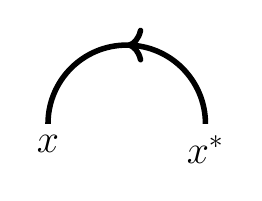
\begin{tikzpicture}[line width=2pt]
\draw[->-=.5] (0,0) arc(0:180:1);
\node[below] at (0,0) {\Large $x^*$};\node[below] at (-2,0) {\Large $x$};
\end{tikzpicture}}}}: \1 \to x \ot x^{*}
\quad\text{and}\quad
\ev_x= \vcenter{\hbox{\scalebox{0.6}{
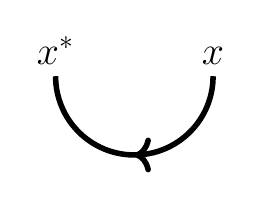
\begin{tikzpicture}[line width=2pt]
\draw[->-=.5] (0,0) arc(0:-180:1);
\node [above] at (0,0) {\Large $x$}; \node [above] at (-2,0) {\Large $x^*$};
\end{tikzpicture}}}}: x^* \ot x \to \1}
%========================================
\newcommand{\EqRigid}{
\vcenter{\hbox{\scalebox{0.6}{
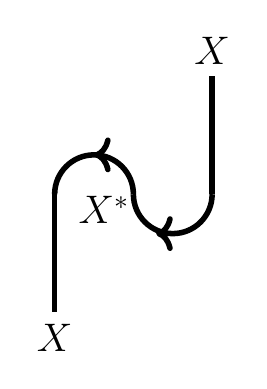
\begin{tikzpicture}[line width=2pt]
\draw (-1,0)--(-1,-1.5); \node[below] at (-1,-1.5) {\Large $X$};
\draw (1,0)--(1,1.5); \node[left] at (0.1,-0.2) {\Large $X^*$};
\draw[->-=.5] (0,0) arc(0:180:0.5); \node[above] at (1,1.5) {\Large $X$};
\draw[-<-=.5] (0,0) arc(180:360:0.5);
\end{tikzpicture}}}} 
\ =
\vcenter{\hbox{\scalebox{0.6}{
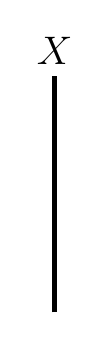
\begin{tikzpicture}[line width=2pt]
\draw (0,0)--(0,3); \node[above] at (0,3) {\Large $X$};
\end{tikzpicture}}}}    
\quad\text{and}\quad
\vcenter{\hbox{\scalebox{0.6}{
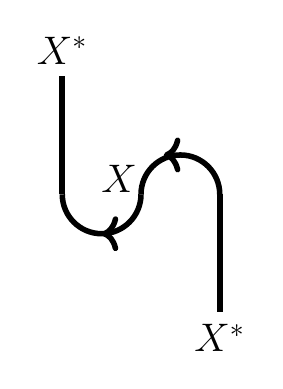
\begin{tikzpicture}[line width=2pt, yscale = -1]
\draw (-1,0)--(-1,-1.5); \node[above] at (-1,-1.5) {\Large $X^*$};
\draw (1,0)--(1,1.5); \node[left] at (0.1,-0.2) {\Large $X$};
\draw[->-=.5] (0,0) arc(0:180:0.5); \node[below] at (1,1.5) {\Large $X^*$};
\draw[-<-=.5] (0,0) arc(180:360:0.5);
\end{tikzpicture}}}} 
\ =
\vcenter{\hbox{\scalebox{0.6}{
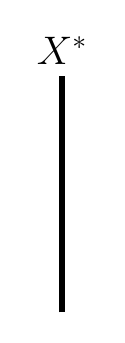
\begin{tikzpicture}[line width=2pt]
\draw (0,0)--(0,3); \node[above] at (0,3) {\Large $X^*$};
\end{tikzpicture}}}}}
%========================================
% Left Quantum dimension 
%========================================
\newcommand{\LQDimPic}{
\vcenter{\hbox{\scalebox{0.6}{
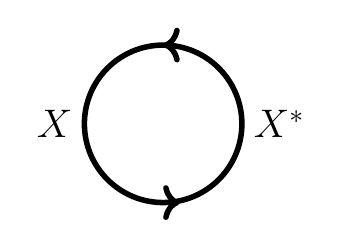
\begin{tikzpicture}[line width=2pt]
\draw[->-=.5] (0,0) arc(0:180:1);
\draw[-<-=.5] (0,0) arc(360:180:1);
\node[left] at (-2,0) {\Large $X$};
\node[right] at (0,0) {\Large $X^*$};
\end{tikzpicture}}}}}
%========================================
% Right Quantum dimension 
%========================================
\newcommand{\RQDimPic}{
\vcenter{\hbox{\scalebox{0.6}{
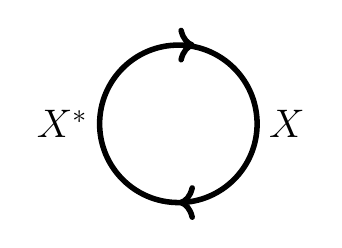
\begin{tikzpicture}[line width=2pt]
\draw[-<-=.5] (0,0) arc(0:180:1);
\draw[->-=.5] (0,0) arc(360:180:1);
\node[left] at (-2,0) {\Large $X^*$};
\node[right] at (0,0) {\Large $X$};
\end{tikzpicture}}}}}
%========================================
% Braiding and its inverse
%========================================
\newcommand{\Brd}{
\vcenter{\hbox{\scalebox{0.6}{
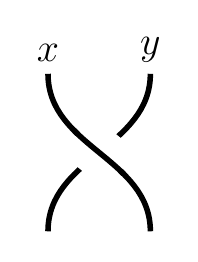
\begin{tikzpicture}[line width=2pt]
\begin{knot}  
\strand[out=down,in=up] (0,0) to (1.3,-2);
\strand[out=down,in=up] (1.3,0) to (0,-2);
\node[above] at (0,0) {\Large  $x$};
\node[above] at (1.3,0) {\Large  $y$};
\end{knot}
\end{tikzpicture}}}}}
\newcommand{\BrdInv}{\vcenter{\hbox{\scalebox{0.6}{
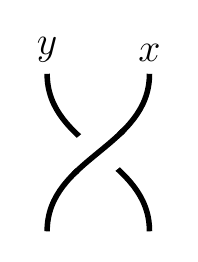
\begin{tikzpicture}[line width=2pt]
\begin{knot}[yscale=-1]  
\strand[out=down,in=up] (0,0) to (1.3,-2);
\strand[out=down,in=up] (1.3,0) to (0,-2);
\node[above] at (0,-2) {\Large  $y$};
\node[above] at (1.3,-2) {\Large  $x$};
\end{knot}
\end{tikzpicture}}}}}
%========================================
% Trivalent Vertex Check 
%========================================
\newcommand{\BranchUp}[1]{
\begin{scope}[shift={#1}]
\draw (0,0) -- ++(45:1.5)
      (0,0) -- ++(135:1.5)
      (0,0) -- (0,-1);
\draw ([shift=(45:0.3cm)]0,0) arc (45:135:0.3cm);
\fill[black] (0,0) circle (3pt);
\end{scope}}
\newcommand{\TrivalentVertexCheck}{
\vcenter{\hbox{\scalebox{0.6}{
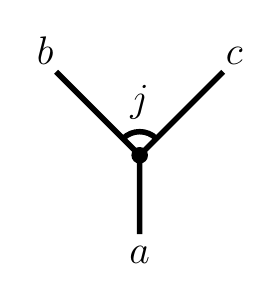
\begin{tikzpicture}[line width=2pt]
\draw (0,0) -- ++(45:1.5)
      (0,0) -- ++(135:1.5)
      (0,0) -- (0,-1);
\draw ([shift=(45:0.3cm)]0,0) arc (45:135:0.3cm);
\fill[black] (0,0) circle (3pt);
\node[above] at (0,0.3) {\Large $j$};
\node[above] at (-1.2, 1) {\Large $b$};
\node[above] at (1.2, 1) {\Large $c$};
\node[below] at (0, -1) {\Large $a$};
\end{tikzpicture}}}}}
%========================================
% Trivalent Vertex Hat
%========================================
\newcommand{\BranchDown}[1]{
\begin{scope}[shift={#1}]
\draw (0,0)--(-1,-1); \draw (0,0)--(1,-1);
\draw ([shift=(225:0.3cm)]0,0) arc (225:315:0.3cm);
\fill[black] (0,0) circle (3pt);
\end{scope}}
\newcommand{\TrivalentVertexHat}{
\vcenter{\hbox{\scalebox{0.6}{
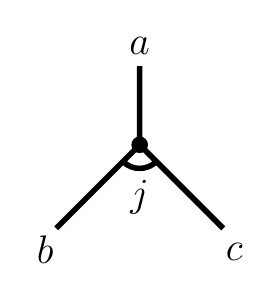
\begin{tikzpicture}[line width=2pt]
\draw (0,0) -- ++(225:1.5)
      (0,0) -- ++(315:1.5)
      (0,0) -- (0,1);
\draw ([shift=(225:0.3cm)]0,0) arc (225:315:0.3cm);
\node[below] at (0,-0.3) {\Large $j$};
\node[below] at (-1.2, -1) {\Large $b$};
\node[below] at (1.2, -1.1) {\Large $c$};
\node[above] at (0, 1) {\Large $a$};
\fill[black] (0,0) circle (3pt);
\end{tikzpicture}}}}}
%========================================
% Straight line (can change label)
%========================================
\newcommand{\StraightLine}[1]{
\vcenter{\hbox{\scalebox{0.6}{
\begin{tikzpicture}[line width=2pt]
\draw (0,0) -- (0,3);
\node[above] at (0,3) {\Large $#1$};
\end{tikzpicture}}}}}
%========================================
%  \ /
%   |   Cup then cap
%  / \               
%========================================
\newcommand{\CupCap}{
\vcenter{\hbox{\scalebox{0.6}{
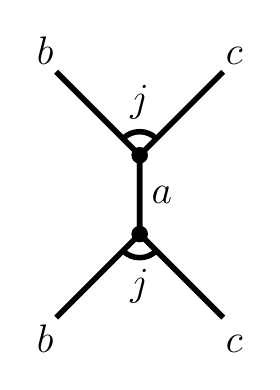
\begin{tikzpicture}[line width=2pt]
\draw (0,0) -- ++(45:1.5)
      (0,0) -- ++(135:1.5)
      (0,0) -- (0,-1);
\draw ([shift=(45:0.3cm)]0,0) arc (45:135:0.3cm);
\node[above] at (0,0.3) {\Large $j$};
\node[above] at (-1.2, 1) {\Large $b$};
\node[above] at (1.2, 1) {\Large $c$};
\fill[black] (0,0) circle (3pt);
\node[right] at (0,-0.5) {\Large $a$};
%%%%%%%%%%%%%%%%%%%%%%%%%%%%%%%%%%%%%%%%%%%
\draw (0,-1) -- ++(225:1.5)
      (0,-1) -- ++(315:1.5)
      (0,-1) -- (0,0);
\draw ([shift=(225:0.3cm)]0,-1) arc (225:315:0.3cm);
\node[below] at (0,-1.3) {\Large $j$};
\node[below] at (-1.2, -2) {\Large $b$};
\node[below] at (1.2, -2.13) {\Large $c$};
\fill[black] (0,-1) circle (3pt);
\end{tikzpicture}}}}}
%========================================
%  |
% / \ 
% \ /   Cap then cup 
%  |
%========================================
\newcommand{\CapCup}{
\vcenter{\hbox{\scalebox{0.6}{
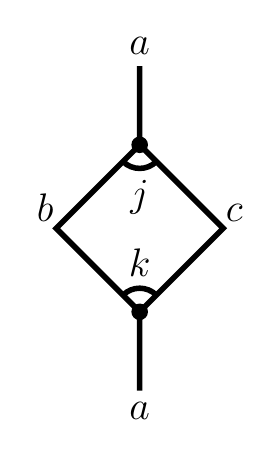
\begin{tikzpicture}[line width=2pt]
\draw (0,0) -- ++(45:1.5) -- ++(135:1.5) node(a1){} 
        -- ++(90:1) node(a2){}
      (0,0) -- ++(135:1.5) -- ++(45:1.5)
      (0,0) -- (0,-1);
\draw ([shift=(45:0.3cm)]0,0) arc (45:135:0.3cm);
\draw (a1) +(225:0.3cm) arc (225:315:0.3cm);
\node[above] at (0,0.3) {\Large $k$};
\node[above] at (-1.2, 1) {\Large $b$};
\node[above] at (1.2, 1) {\Large $c$};
\fill[black] (0,0) circle (3pt);
\fill[black] (a1) circle (3pt);
\node[below] at (0,-1) {\Large $a$};
\node[above] at (a2) {\Large $a$};
\node[below] at ($(a1) + (0,-0.3)$) {\Large $j$};
\end{tikzpicture}}}}}
%========================================
% holes with curves
%========================================
\newcommand{\HoleWithCurve}[1]{
\begin{scope}[shift={#1}]
\hole{0,-0.5};
\draw[purple] (0, 0.21) arc (-90:90:0.3 and 0.87);
\draw[purple, dashed] (0, 0.21) arc (270:90:0.3 and 0.87);
\draw[blue] (0,0) ellipse (1.2 and 0.6);
\end{scope}}
%========================================
\newcommand{\LeftEquator}[1]
{\begin{scope}[shift={#1}]
\draw[Green] (0.48,0) arc (180:90:1.52 and 0.6);
\draw[Green, dashed] (0.48,0) arc (180:270:1.52 and 0.6);    
\end{scope}}
%========================================
\newcommand{\RightEquator}[1]{
\begin{scope}[shift={#1}]
\draw[Green] (-0.48,0) arc (0:90:1.52 and 0.6);
\draw[Green, dashed] (-0.48,0) arc (0:-90:1.52 and 0.6);        
\end{scope}}
%========================================
% Hopf link
%========================================
\newcommand{\HopfLink}[1]{\vcenter{\hbox{\scalebox{0.6}{
\begin{tikzpicture}[line width=2pt]
\begin{scope}[shift={#1}]
\draw (0,0) arc (0:180:0.5 and 1);  
\draw (0,1.5) arc (360:180:0.5 and 1);
\fill[white] (-0.18,0.73) circle (3pt);  
\fill[white] (-0.82,0.73) circle (3pt);  
\draw (0,0) arc (0:90:0.5 and 1);  
\draw (-0.5,0.5) arc (270:180:0.5 and 1);
\draw(-0.55,1)--++(0.2,0.13);\draw (-0.55,1)--++(0.16,-0.2);
\draw(-0.45,0.5)--++(-0.13,0.18);\draw(-0.45,0.5)--++(-0.18,-0.13);
\end{scope}
\end{tikzpicture}}}}}





\renewcommand{\hole}[1]{
\draw ([shift=(45:0.707)]$(#1)$) arc (45:135:0.707);
\draw ([shift=(210:0.707)]$(#1)+(0,1)$) arc (210:330:0.707)
}

\newcommand{\grayhole}[1]{
\draw[gray] ([shift=(45:0.707)]$(#1)$) arc (45:135:0.707);
\draw[gray] ([shift=(210:0.707)]$(#1)+(0,1)$) arc (210:330:0.707)
}



































































